\documentclass[11pt, titlepage]{article}
% Common packages/environments to remove clutter

% Packages
\usepackage[utf8]{inputenc}
\usepackage{amsmath, amsfonts, amssymb, amsthm, enumitem, tikz, import, mathtools}
\usepackage[
  top=2cm,
  bottom=2cm,
  left=3cm,
  right=3cm,
  headheight=17pt,
  includehead, includefoot,
  heightrounded,
]{geometry}

% Problem environment
\newtheoremstyle{emptyplain}
    {}          % default space above
    {}          % default space below
    {}          % default body font
    {}          % no indent
    {\bfseries} % head font
    {.}         % punctuation after theorem head
    { }         % space after theorem head
    {#3}
\theoremstyle{emptyplain}
\newtheorem*{problem}{}

% Solution Environment
\newenvironment{solution}{
  \begin{proof}[Solution]
    \vspace{-2px}
    \setlength{\parskip}{4px}
    \setlength{\parindent}{0px}
}{
\end{proof}
}

\usepackage{fancyhdr, float}
\usepackage[
    top=2cm,
    bottom=2cm,
    left=3cm,
    right=3cm,
    headheight=17pt,
    includehead, includefoot, heightrounded,
]{geometry}

% Header
\pagestyle{fancy}
\fancyhf{}
\lhead{Math 2552 Final Exam Makeup Part B}
\rhead{Akash Narayanan}

% Opening
\title{Math 2552 Final Exam Makeup Part B}
\author{Akash Narayanan}
\date{May 7, 2021}

\begin{document}
    \maketitle

    \begin{enumerate}
        % Problem 1
        \item (10 points) Use the variation of parameters method to identify the general solution to
        \[
        \vec{x}' =
        \begin{pmatrix}
            2 & -1 \\
            -1 & 2
        \end{pmatrix} \vec{x} +
        \begin{pmatrix}
            2e^{3t} \\
            -4e^{3t}
        \end{pmatrix}.
        \]
        Please show your work.

        \begin{solution}
            We start by finding the solution to the homogeneous equation to identify a fundamental set of solutions.
            Letting $A$ denote the coefficient matrix, we find
            \[
            \det
            \begin{pmatrix}
                2 - \lambda & -1 \\
                -1 & 2 - \lambda
            \end{pmatrix} =
            \lambda^2 - 4 \lambda + 3 = (\lambda - 1) (\lambda - 3) = 0
            \]
            so the eigenvalues are $\lambda_1 = 1$ and $\lambda_2 = 3$.
            Now we find the corresponding eigenvectors by solving $(A - \lambda I) \vec{v} = 0$.
            \begin{gather*}
                \begin{pmatrix}
                    1 & -1 \\
                    -1 & 1
                \end{pmatrix} \vec{v}_1 = 0 \\
                \Longrightarrow
                \vec{v}_1 =
                \begin{pmatrix}
                    1 \\
                    1
                \end{pmatrix}
            \end{gather*}
            and
            \begin{gather*}
                \begin{pmatrix}
                    -1 & -1 \\
                    -1 & -1
                \end{pmatrix} \vec{v}_2 = 0 \\
                \Longrightarrow
                \vec{v}_2 =
                \begin{pmatrix}
                    1 \\
                    -1
                \end{pmatrix}
            \end{gather*}
            Then the solution to the homogeneous equation is
            \[
            \vec{x} = c_1 e^{t}
            \begin{pmatrix}
                1 \\
                1
            \end{pmatrix} + c_2 e^{3t}
            \begin{pmatrix}
                1 \\
                -1
            \end{pmatrix}
            \]
            The corresponding fundamental matrix is
            \[
            X =
            \begin{pmatrix}
                e^t & e^{3t} \\
                e^t & -e^{3t}
            \end{pmatrix}
            \]
            We calculate the determinant and inverse.
            \begin{gather*}
                \det(X) = -e^{4t} - e^{4t} = -2e^{4t} \\
                X^{-1} = \frac{1}{\det(Y)}
                \begin{pmatrix}
                    -e^{3t} & -e^{3t} \\
                    -e^{t} & e^{t}
                \end{pmatrix} = \frac{1}{2}
                \begin{pmatrix}
                    e^{-t} & e^{-t} \\
                    e^{-3t} & -e^{-3t}
                \end{pmatrix}
            \end{gather*}
            Then a particular solution is given by
            \[
            x_p = X \int Y^{-1} g dt
            \]
            where $g$ is the nonhomogeneous part of the system of differential equations. We find
            \begin{align*}
                x_p &= \frac{1}{4} X \int
                \begin{pmatrix}
                    e^{-t} & e^{-t} \\
                    e^{-3t} & -e^{-3t}
                \end{pmatrix}
                \begin{pmatrix}
                    2e^{3t} \\
                    -4e^{3t}
                \end{pmatrix} dt \\
                &= \frac{1}{4} X \int
                \begin{pmatrix}
                    -2e^{2t} \\
                    6
                \end{pmatrix} dt \\
                &= \frac{1}{4}
                \begin{pmatrix}
                    e^t & e^{3t} \\
                    e^t & -e^{3t}
                \end{pmatrix}
                \begin{pmatrix}
                    -e^{2t} \\
                    6t
                \end{pmatrix} \\
                &= \frac{1}{4}
                \begin{pmatrix}
                    (6t - 1) e^{3t} \\
                    (-6t - 1) e^{3t}
                \end{pmatrix}
            \end{align*}
            Finally, we have the general solution to the system of equations is
            \[
            \vec{x} = c_1 e^t
            \begin{pmatrix}
                1 \\
                1
            \end{pmatrix}
            + c_2 e^{3t}
            \begin{pmatrix}
                1 \\
                -1
            \end{pmatrix}
            + \frac{1}{4}
            \begin{pmatrix}
                (6t - 1) e^{3t} \\
                (-6t - 1) e^{3t}
            \end{pmatrix}
            \]
        \end{solution}

        \pagebreak

        % Problem 2
        \item (10 points) Consider the non-linear system below.
        \[
        \frac{dx}{dt} = y^2 - 1, \quad \frac{dy}{dt} = x + y - 1
        \]

        \begin{enumerate}[label={(\alph*)}]
            \item Plot and label the nullclines of the system. Please label your axes.

            \item Identify all critical points of the system. Show your work.

            \item Compute the Jacobian matrix.
            For each critical point you identified in part (b), use eigenvalues to classify the critical points according to stability (stable, unstable, asymptotically stable) and type (saddle, proper node, etc).
        \end{enumerate}

        \begin{solution}
            The nullclines are the set of points where the derivatives are equal to zero.
            That is, the $x$-nullcline is given by the equation $y^2 = 1$ and the $y$-nullcline is given by the equation $y = 1 - x$.
            These can be seen in the graph below, where the $x$-nullcline is in red and the $y$-nullcline is in green.
            \begin{figure}[H]
                \centering
                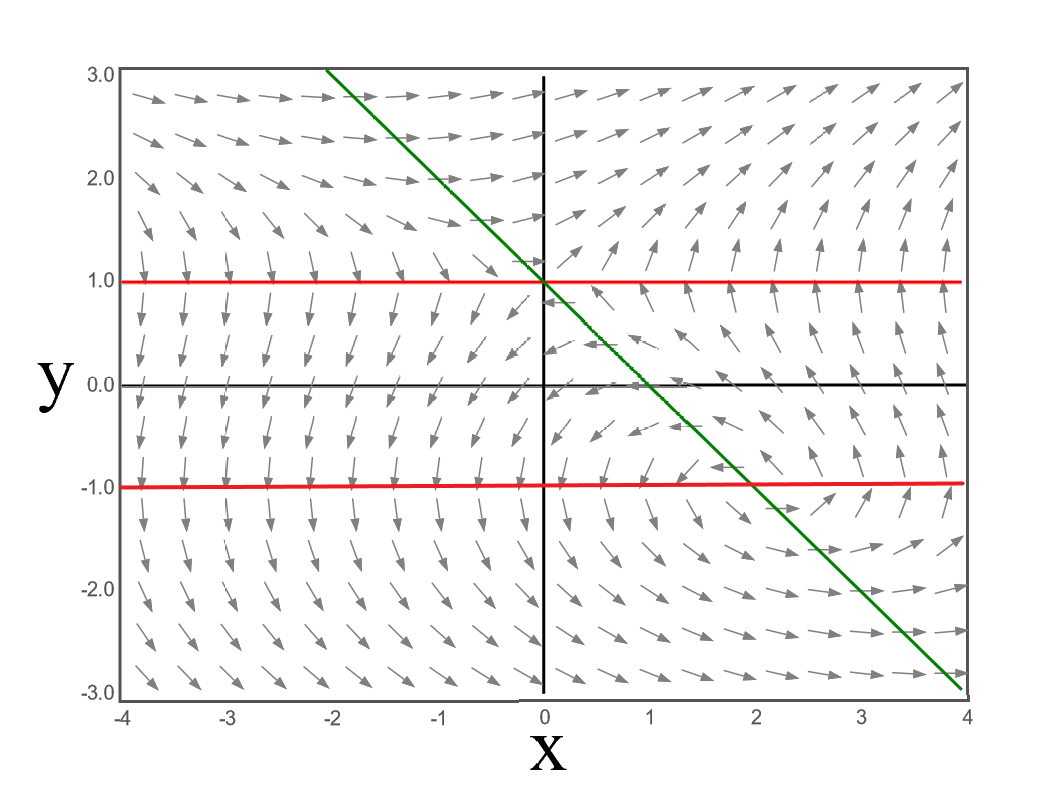
\includegraphics[width=0.8\textwidth]{media/slopeField.png}
            \end{figure}

            The critical points are the points where nullclines intersect. For the given non-linear system, if $y = -1$ then $-1 = 1 - x$ so $x = 2$, meaning $(2, -1)$ is a critical point.
            The other critical point occurs when $y = 1$, so $1 = 1 - x$ and $x = 0$, meaning the other critical point is $(0, 1)$.

            We now compute the Jacobian matrix.
            \[
            J =
            \begin{pmatrix}
                \frac{\partial x'}{\partial x} & \frac{\partial x'}{\partial y} \\
                \frac{\partial y'}{\partial x} & \frac{\partial y'}{\partial y}
            \end{pmatrix} =
            \begin{pmatrix}
                0 & 2y \\
                1 & 1
            \end{pmatrix}
            \]
            We now use the Jacobian to classify the critical points identified above.
            \begin{gather*}
                J(2, -1) =
                \begin{pmatrix}
                    0 & -2 \\
                    1 & 1
                \end{pmatrix} \Longrightarrow
                (-\lambda)(1 - \lambda) + 2 = \lambda^2 - \lambda + 2 = 0 \\
                \Longrightarrow \lambda = \frac{1 \pm \sqrt{-7}}{2}
            \end{gather*}
            Since both eigenvalues are complex with real part greater than zero, the critical point $(2, -1)$ is an unstable node.
            \begin{gather*}
                J(0, 1) =
                \begin{pmatrix}
                    0 & 2 \\
                    1 & 1
                \end{pmatrix} \Longrightarrow
                (-\lambda)(1 - \lambda) - 2 = \lambda^2 - \lambda - 2 = 0 \\
                \Longrightarrow \lambda = -1, 2
            \end{gather*}
            Since both eigenvalues are real, one being negative and the other positive, the critical point $(0, 1)$ is a saddle.
        \end{solution}

        \pagebreak

        % Problem 3
        \item (5 point) A tank holds 200 litres of salt water.
        Initially, there are 2 kg of salt in the tank.
        Salt water containing 0.2 kg of salt per litre is pumped into the tank at a rate of litres per minute.
        The well-mixed solution is pumped out at a rate of 0.5 litres per minute.
        Construct an initial value problem that models the amount of salt in the tank for $t \in [0, T]$, where $T$ is some positive constant.
        Do not solve your initial value problem.

        \begin{solution}
            Let $x(t)$ be the amount of salt in the tank at time $t$.
            The initial condition states that $x(0) = 2 kg$.
            Let $V(t)$ be the amount of water in the tank at time $t$ so that $V(t) = 4t - 0.5t = 3.5t$.
            Then we find
            \begin{align*}
                \frac{dx}{dt} &= (0.2 \text{ kg/L} \cdot 4 \text{ L/min}) - \left(\frac{x}{V(t)} \text{ kg/L} \cdot 0.5 \text{ L/min}\right) \\
                &= 0.8 - \frac{x}{7t}
            \end{align*}
            This equation models the amount of salt in the tank for $t \in [0, T]$ where $T$ represents the time when the tank is full.
            This occurs when $3.5T = 200$ or $T \approx 57.14 \text{ min}$.
        \end{solution}

        \pagebreak

        % Problem 4
        \item (4 points) Construct an initial value problem for the following situation.

        A 0.1 Newtons (N) force stretches a spring 0.01 m.
        A mass weighing 4 kg is attached to the spring, and the spring is also attached to a viscous damper that applies a force of 0.6 N when the velocity of the mass is 0.1 m/s. The mass is pulled up 0.1 m above its equilibrium position and given an initial upward velocity of 0.12 m/s.

        \begin{solution}
            The 0.1 N force which stretches the spring 0.01 m tells us that the spring constant is $k = 0.1$ since $F = kx$.
            Furthermore, the damping constant is $b = 6$ since $F = bv$.
            The sum of all forces acting on the system should equal 0 since there are no outside forces.
            Thus, we find
            \[
            4x'' - 6x' - 0.1x = 0
            \]
            where the downward direction is positive. The initial conditions are $x(0) = -0.1$ and $x'(0) = -0.12$.
        \end{solution}

        \pagebreak

        % Problem 5
        \item (10 points) Use the Laplace transform to solve the IVP.
        \[
        y'' - 3y' + 2y = 20e^{3t}, \quad y(0) = 5, \quad y'(0) = 4
        \]

        \begin{solution}
            Taking the Laplace transform of both sides gives
            \[
            (s^2 Y - sy(0) - y'(0)) - 3(sY - y(0)) + 2Y = \frac{20}{s - 3}
            \]
            Simplifying and rearranging yields
            \[
            Y(s) = \frac{5s^2 - 26s + 53}{s^3 - 6s^2 + 11s - 6} = \frac{5s^2 - 26s + 53}{(s-1) (s-2) (s-3)}
            \]
            The partial fraction decomposition of the right side is
            \[
            \frac{16}{s - 1} - \frac{21}{s - 2} + \frac{10}{s - 3}
            \]
            Taking the inverse Laplace transform of this gives
            \[
            y(t) = 16e^{t} - 21e^{2t} + 10e^{3t}
            \]
        \end{solution}

    \end{enumerate}
\end{document}
